\subsection{Galaxy Number Counts}

\begin{figure}
    \centering
    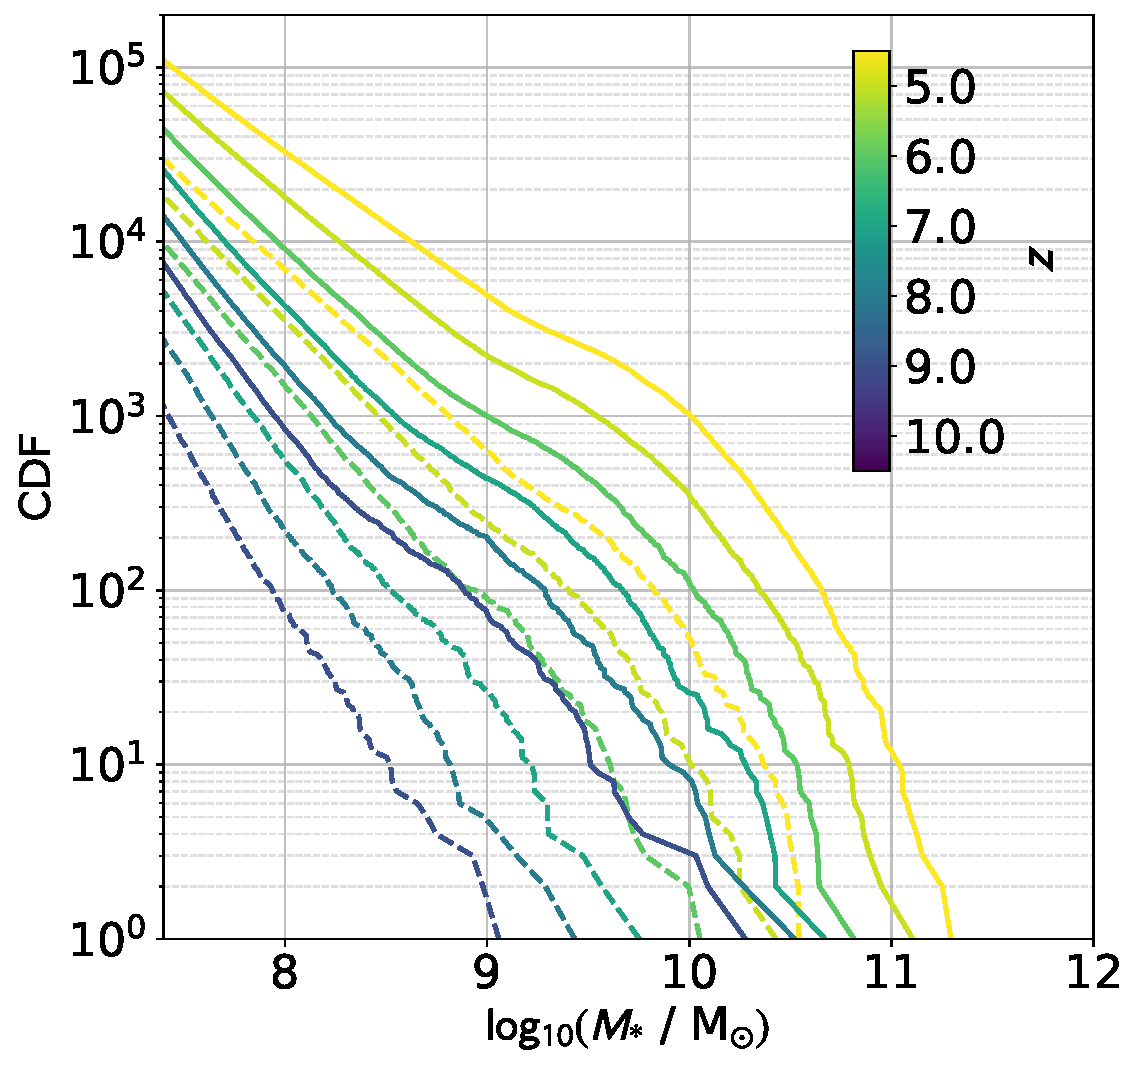
\includegraphics[width=\columnwidth]{images/compare_cumulative.pdf}
    \caption{Cumulative distribution of stellar masses for all \flares\ regions combined (solid) and the fiducial \eagle\ Reference volume (dashed).}
    \label{fig:comp_hist}
\end{figure}

We begin by showing the raw number counts of galaxies.
\fig{comp_hist} shows the cumulative distribution function of galaxies with stellar mass for both \flares\ and the Reference periodic volume ($V = (100 \, \mathrm{cMpc})^3$).
We produce over $\sim 20$ times more $10^{10} \, \mathrm{M_{\odot}}$ galaxies at $z = 5$ than obtained in the 100\,cMpc periodic volume, despite the fact that the total high-resolution volume of all resimulated regions is only 50\% larger than the periodic volume.
This confirms that the first galaxies are significantly biased to high overdensity regions.
